\documentclass[a4paper,11pt]{article}
% Use ctrl + alt + V to view live pdf

% Packages
\usepackage[utf8]{inputenc} % For encoding
\usepackage[T1]{fontenc} % Better handling of accented characters and hyphenation
\usepackage{microtype} % Improves spacing and justification
\usepackage{amsmath, amssymb} % For equations and symbols
\usepackage{graphicx} % For including graphics/images
\usepackage{caption} % For customizing figure and table captions
\usepackage{subcaption} % For subfigures and subcaptions
\usepackage{float} % For fixing figure and table positions
\usepackage{booktabs} % For professional-looking tables
\usepackage{siunitx} % For consistent typesetting of units and numbers
\usepackage[margin=2cm]{geometry} % Adjusts page margins
\usepackage{fancyhdr} % For custom headers and footers
\usepackage{lmodern} % For a professional-looking font (main body font)
\usepackage{titlesec} % For title customization
\usepackage{array} % For custom table formatting
\usepackage[colorlinks=true, linkcolor=black, citecolor=blue, urlcolor=blue]{hyperref} % Colored links without boxes
\usepackage{cleveref} % For improved cross-referencing    
\usepackage{multirow}
\usepackage{enumitem}
\usepackage{listings}
\usepackage{xcolor}
\usepackage{textcomp}
\usepackage{tabularx}
\usepackage{changepage}
\usepackage{tikz}
\usepackage{pdfpages}
\usepackage[table]{xcolor}
\usepackage{tocloft}

% Reduce spacing between entries
\setlength{\cftbeforesecskip}{1em}
\setlength{\cftbeforesubsecskip}{1em} 
\setlength{\cftbeforesubsubsecskip}{1em}

\usetikzlibrary{shapes.geometric, arrows}
% --- C++ Style ---
\lstdefinestyle{cpp-style}{
    language=C++,
    basicstyle=\ttfamily\footnotesize,
    keywordstyle=\color{red}\bfseries,
    stringstyle=\color{orange},
    commentstyle=\color{green!70!black}\itshape,
    identifierstyle=\color{blue},
    numbers=left,
    numberstyle=\tiny\color{gray},
    numbersep=10pt,
    backgroundcolor=\color{white},
    showspaces=false,
    showstringspaces=false,
    breaklines=true,
    breakatwhitespace=true,
    tabsize=4,
    captionpos=b,
    frame=single,
    rulecolor=\color{black},
}

% --- Python Style ---
\lstdefinestyle{python-style}{
    language=Python,
    basicstyle=\ttfamily\footnotesize,
    keywordstyle=\color{red}\bfseries,
    commentstyle=\color{green!70!black}\itshape,
    stringstyle=\color{orange},
    identifierstyle=\color{blue},
    numbers=left,
    numberstyle=\tiny\color{gray},
    numbersep=8pt,
    backgroundcolor=\color{white},
    showstringspaces=false,
    showspaces=false,
    breaklines=true,
    breakatwhitespace=true,
    tabsize=4,
    captionpos=b,
    frame=single,
    rulecolor=\color{black},
}

\renewcommand{\lstlistingname}{Program}
% Custom settings
\pagestyle{fancy}
\fancyhf{}
\fancyhead[L]{\textit{SF4 - DataLogger}} % Header left
\fancyhead[R]{\textit{Will Hewes - wh365}} % Header right 
\fancyfoot[C]{\thepage} % Footer center
\setlength{\headheight}{15pt} % Header height
\setlength{\parindent}{0em} % Indentation for paragraphs
\setlength{\parskip}{0.5em} % Add spacing between paragraphs
\setlength{\abovedisplayskip}{1em}
\setlength{\belowdisplayskip}{1em}
\setlength{\abovedisplayshortskip}{1em}
\setlength{\belowdisplayshortskip}{1em}
% \setlist{topsep=0.2em, partopsep=0em, itemsep=0.1em, parsep=0em}

\graphicspath{{Images/}}

% \renewcommand{\arraystretch}{1.2}

% Title formatting
\renewcommand{\maketitle}{
    \begin{center}
        \LARGE \textbf{ENGINEERING TRIPOS PART IIA} \\[0.5em]
        \Large \textbf{SF4 - DataLogger} \\
        \textbf{Final Report} \\
        \small Will Hewes - wh365 \\ 
        Pembroke College \\ 
        \vspace{0.5em}
    \end{center}
}

\begin{document}
\pagenumbering{gobble}
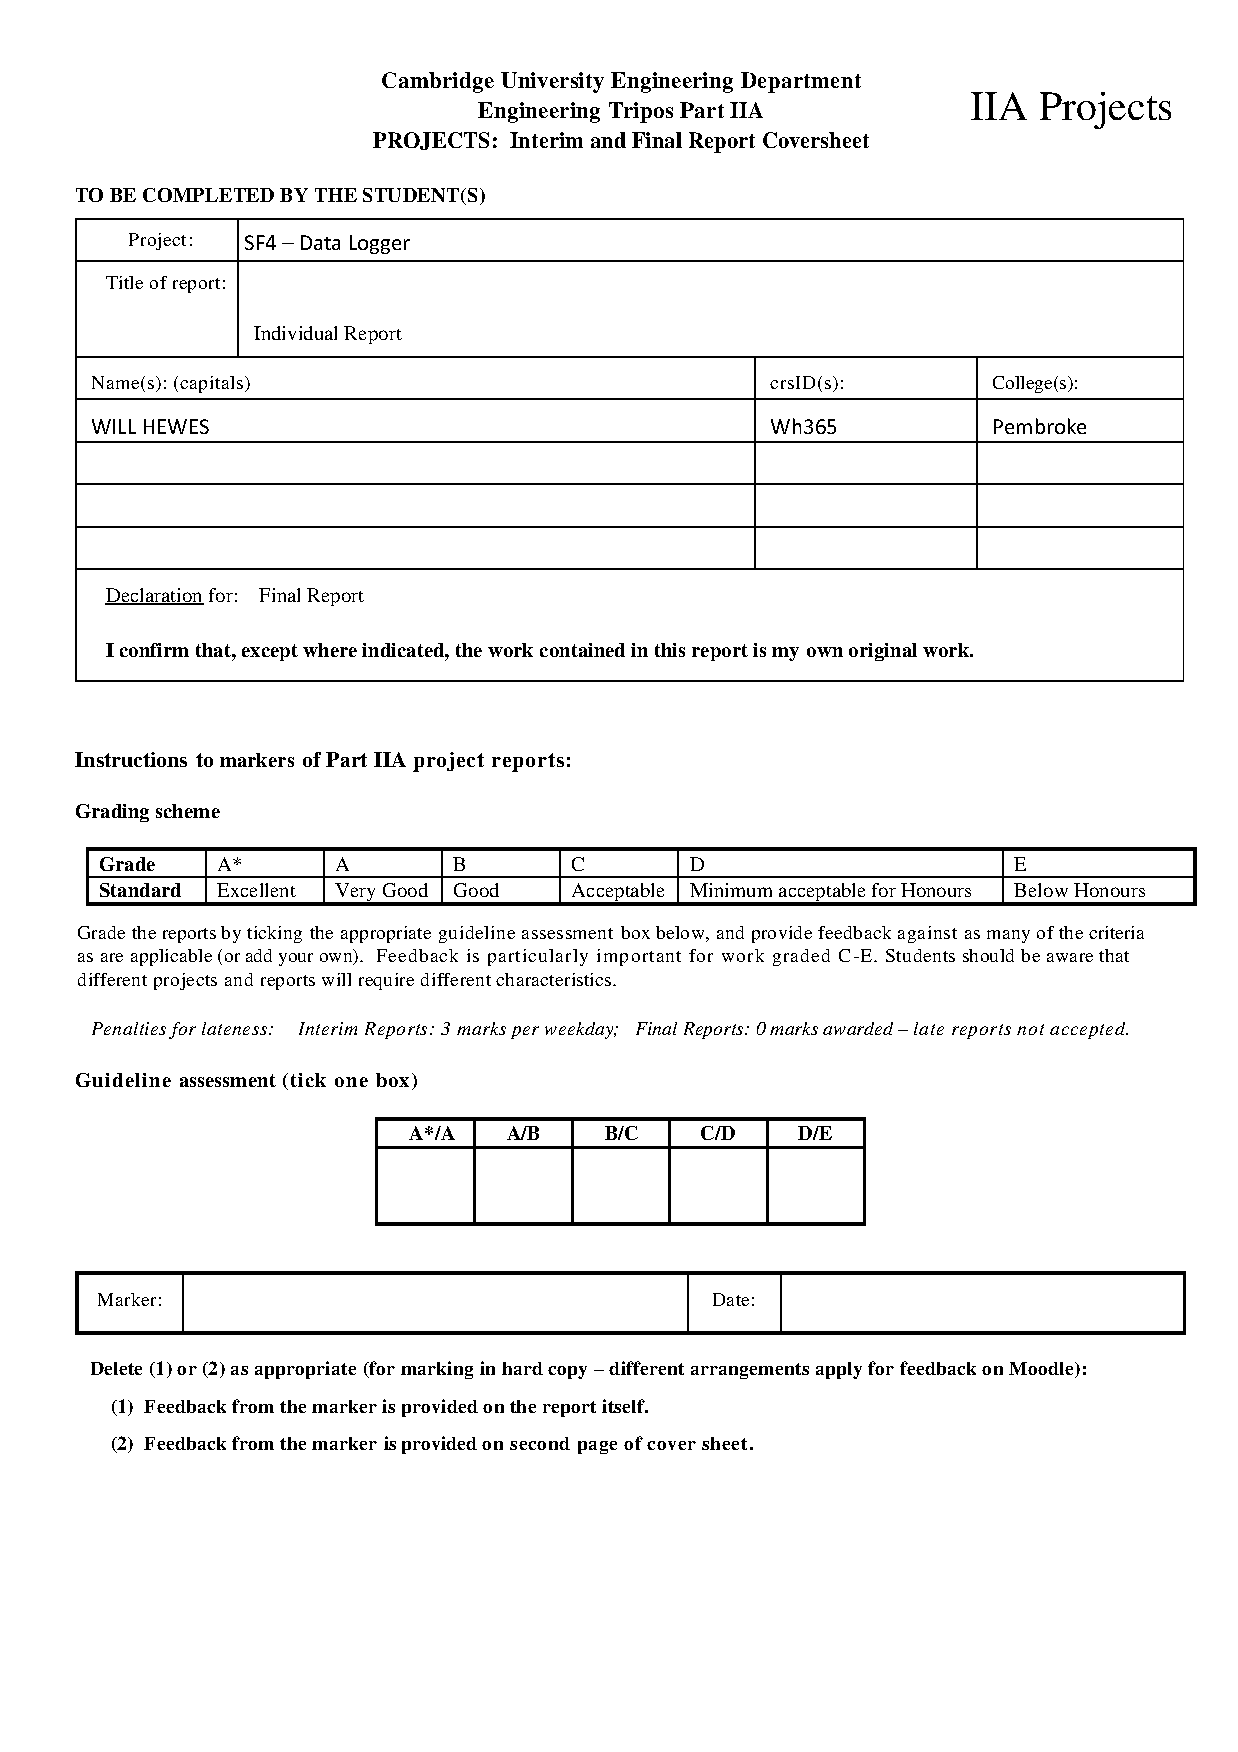
\includepdf[pages=-]{Handouts/IIA_Project_Coversheet Final Report.pdf}
\maketitle
\hrule
\tableofcontents
\newpage
\pagenumbering{arabic} \setcounter{page}{1}

\section{Introduction}
\label{sec:introduction}

The aim of this project was to develop a microcontroller-based 
automatic plant watering system.
The system can autonomously monitor soil moisture levels, 
plot the data over time, and provide options to water the plant
manually when required or in response to threshold moisture levels.
This allows for effective monitoring and care with minimal user intervention.

In addition to moisture sensing, the system also tracks temperature, 
and was supposed to track humidity and light -
though this could not be implemented due to component delivery delays.
This means most of the key factors affecting plant health
can be closely tracked, enabling detailed analysis of
optimum conditions for plant health.
These additional features enhance the system's utility for targeted care for the plants,
or for more sophisticated control and research.

The motivation behind creating this autonomous watering system was twofold. 
Firstly, it can be used as demonstrated on a small scale,
allowing direct control over the conditions of one 
or a small number of houseplants,
offering a convenient way to care for plants.
This will remove the majority of the care required
to look after these often frail plants,
which is particularly useful over holidays or 
during the hot Summer months.
As a university student with several well-loved plants,
this has immediate personal appeal.

On a larger scale, the system provides a modular, 
low-cost framework adaptable to industrial or agricultural applications, 
where automated irrigation and environmental monitoring are increasingly valuable.
The low cost and simple design of the system will be appealing 
to widespread, versatile integration,
and the ease with which components can be added
and the GUI can be customised will allow for rapid expansion into various sectors.

\section{System Summary}
\label{sec:summary}

The final system comprises a microcontroller
connected via USB serial to a Python-based PC interface. 
The microcontroller collects real-time data from a capacitive soil moisture sensor 
and a TMP36 temperature sensor, formats the data, 
and transmits it at regular, rapid intervals. 
The PC software receives the data, displays it graphically, 
and writes it to a timestamped CSV log.

The watering mechanism is controlled by a mini servo motor 
which actuates a 3D-printed pinch valve connected to a reservoir. 
Watering can be triggered manually from the graphical user interface, 
or automatically when the measured soil moisture drops below 
a configurable threshold. 
This enables a complete closed-loop feedback system 
between environmental sensing, control logic, 
and physical actuation.

The GUI also provides users with real-time feedback, 
warning indicators for out-of-range values, 
and basic controls for adjusting system thresholds and modes. 
Operation is intended to be simple, low-maintenance, 
and suitable for unattended deployment over extended periods.

While targeted toward small-scale domestic use, 
the system's modular design allows for straightforward expansion. 
Additional sensors (e.g., humidity, light, air quality), 
alternative actuators, or wireless communication modules 
can be added with minimal reconfiguration, 
making the platform a flexible basis for 
larger agricultural or environmental monitoring systems.

\section{Project Management}
\label{sec:project_management}

The project was developed collaboratively in a two-person team, 
with both members working on the system holistically,
applying changes to each module incrementally
as the product was slowly developed.
This approach was taken as opposed to a divided approach -
wherein each member would manage either software or firmware -
with the intention of giving each of us a better understanding 
and overview of the system as a whole,
allowing us to effectively contribute ideas 
concerning the whole project collaboratively. 

This had the consequence that on occasion we would 
both be making changes to the same module simultaneously.
By nature of this development style,
there was an increased risk of conflicts introduced to the system
if we did not take proper care to ensure that our changes were compatable.
As a result, version control and clear communication 
became a vital aspect of our project management.

Version control and collaborative development were managed using GitHub, 
enabling parallel work on the codebase
and simplifying the process of merging changes and tracking development history. 
This also allowed modular elements - 
such as the GUI framework and firmware routines -
to be developed and tested in isolation before being brought together.

The project followed a phased development structure:
\begin{enumerate}[nosep]
    \item \textbf{Component Validation:} 
    Initial sessions focused on ordering the individual sensors 
    and actuators then evaluating them through breadboard testing, 
    ensuring reliable signal acquisition and control.
    \item \textbf{Prototype Development:} 
    In parallel with circuit construction, a socket-based simulation 
    of the Arduino-PC interface was created to support 
    early development of the GUI and data parsing routines 
    in the absence of hardware.
    \item \textbf{System Integration and Testing:} 
    Once physical components were functional, development transitioned 
    to serial communication over USB. 
    Modules were progressively integrated and tested together 
    in a final working system.
\end{enumerate}

Throughout the project, care was taken to adopt a modular workflow, 
with each subcomponent independently tested and versioned. 
This reduced the risk of cascading failures during integration and 
supported incremental development even in the face of hardware delays 
or debugging setbacks.

\section{System Architecture}
\label{sec:architecture}

\subsection{Block Diagram}
\label{sec:block_diagram}

Figure \ref{fig:Block_Diagram_for_the_automatic_watering_system} below presents a high-level overview 
of the system architecture, outlining the key components and their interactions. 
At the centre is the Arduino Uno microcontroller, responsible for interfacing with 
the sensors and controlling the servo-driven watering mechanism. 
It collects analogue data from the soil moisture and temperature sensors, 
processes it internally, and transmits formatted readings 
to the host PC via a serial USB connection.

\begin{figure}[H]
    \centering
    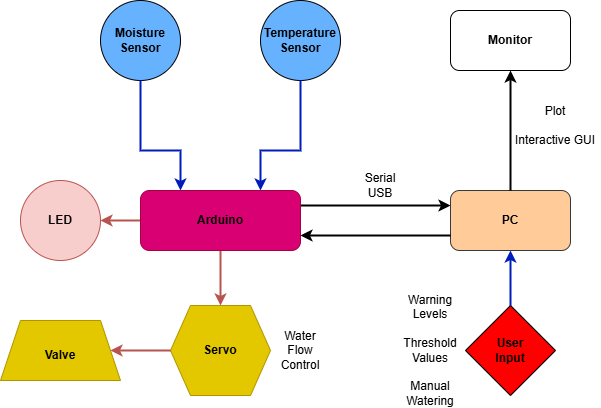
\includegraphics[width=0.6\textwidth]{Datalogger Block Diagram - final.png}
    \caption{Block Diagram for the automatic watering system}
    \label{fig:Block_Diagram_for_the_automatic_watering_system}
\end{figure}

The PC software receives this data stream and handles real-time visualisation
and CSV logging.
The user can configure system parameters through a graphical user interface, 
which sends commands back to the Arduino to adjust moisture thresholds, 
trigger watering, or enable warning indicators.
The servo receives control signals from the Arduino and 
actuates a 3D-printed pinch valve attached to a water reservoir, 
allowing precise water delivery to the plant. 

\subsection{Component Orders}
\label{sec:Components}
The physical system was built around a small set of carefully chosen components, 
ordered through Farnell. 
The sensors included a capacitive soil moisture sensor \cite{dfrobot}, 
chosen due to its improved output stability and longevity compared to a resistive module,
and a TMP36 temperature sensor for simple analogue interfacing \cite{tmp36} \cite{arduino_tmp36}, 
which required a 100pF capacitor acting in parallel between its output pin and the ground
in order to stabilise its readings, 
as well as the incorporation of an \texttt{AREF} wire.

A mini servo motor \cite{arduino_servo} was selected to control the water delivery mechanism, 
providing reliable actuation of a 3D-printed pinch valve \cite{pinch_valve_design}.
This likewise had a capacitor placed between its power and ground pins 
to limit current spikes and provide a smoother, controlled motion.

Additional sensors for humidity and light intensity were also ordered, 
but were not included in the final system due to shipping delays. 
Nonetheless, space was reserved within the system design 
for their future integration.

These components are shown in Table \ref{tab:component_order} in the Appendix,
with the unused sensors highlighted in yellow.
With a budget of £15, there was a remaining £3.65 
that could be used for integration of more sensors,
or replacing current sensors with a higher quality alternative.

\subsection{Circuit Design}
\label{sec:circuit_design}

The final circuit design consisted of a single Arduino Uno board interfacing 
with two analogue sensors and a mini servo motor. The sensors were connected 
to analogue input pins, with the soil moisture sensor wired directly and the 
TMP36 temperature sensor routed through a \SI{100}{\pico\farad} capacitor 
between its signal and ground pins to suppress high-frequency noise,
improving stability of the output signal. 
The Arduino's \texttt{AREF} pin was set to an external \SI{3.3}{\volt} reference 
to improve ADC resolution and match the expected sensor output range.
The servo motor required a \SI{100}{\micro\farad} decoupling capacitor added between 
its power and ground pins to limit voltage dips during actuation.

The complete analogue circuit layout is shown in 
Figure~\ref{fig:Analogue_Circuit_Diagram_for_the_automatic_watering_system}.

\begin{figure}[H]
    \centering
    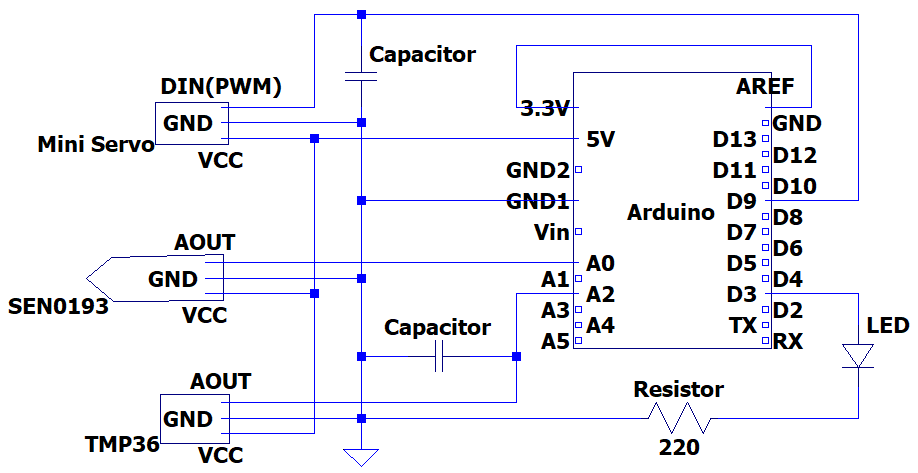
\includegraphics[width=0.6\textwidth]{Analogue Circuit Diagram - final.png}
    \caption{Analogue Circuit Diagram for the automatic watering system}
    \label{fig:Analogue_Circuit_Diagram_for_the_automatic_watering_system}
\end{figure}

\subsection{Watering Mechanism}
\label{sec:water_system}

The water delivery system was implemented using the mini servo motor to actuate a 
3D-printed pinch valve \cite{pinch_valve_design}. 
This design was selected due to its ease of implementation, compact size, 
and small number of parts,
reducing the risk of any mechanical faults within the system. 
The open-source valve design was scaled up 
to fit the PVC tubing we had on hand to connect.

The servo applies a clamping force to compress the tubing, restricting flow when closed 
and releasing it when opened. This mechanism provided a reliable and cost-effective 
alternative to traditional solenoid valves or pump systems, which tend to require 
greater current draw and more complex power handling.
An image of the servo mechanism can be seen in Figure \ref{fig:servo}
in the Appendix.

A moisture threshold, configured via the PC interface, controlled automatic actuation. 
When the measured moisture dropped below this value stored on the Arduino, 
the servo was triggered to open the valve for a set duration, 
delivering a fixed amount of water. 
Manual triggering was also available through the GUI.

The actuation logic, timing, and safety handling are further detailed in 
Section~\ref{sec:firmware}. 

\section{Initial Development}
\label{sec:initial_development}

This section will detail the initial milestone that we set out to achieve.
The intention behind implementing these functionalities
which would subsequently be removed in some cases
was to help build a working baseline which incorporated the sensor readings,
some form of communication, and a basic GUI from which we would build.

\subsection{Sensor Prototyping}
\label{sec:sensor_prototyping}

Upon receiving the sensors and servo motor we had ordered,
the first task would be to get a basic program and output from each of them individually,
working exclusively through the Arduino for now.
This would set a functional output that could then be integrated into other features
and processed as required.
After some small difficulties in setting up these sensors,
detailed in Section \ref{sec:technical_challenges},
we were able to get all the components functioning as required.

\subsection{GUI}
\label{sec:gui_simulation}

Before hardware testing was complete, a preliminary graphical user interface was created 
to simulate the output of the final control system. 
At this stage, the sensor values were simulated using a local socket stream, mimicking 
the serial data that would later be sent by the Arduino. This enabled us to build and 
refine key features such as real-time sensor measurements,
fixed width graph plotting, and threshold adjustment widgets.

This early GUI prototype, developed in Tkinter, would serve as the structural 
foundation of the final interface, providing an object-oriented architecture 
onto which features could be added modularly as development progressed.
In later versions, we would switch over to PySide6,
building from a similar framework but allowing 
more customisation and responsiveness.

The GUI for this preliminary design can be seen in 
Figures \ref{fig:prelim_GUI_readings} and \ref{fig:prelim_GUI_plot} in the Appendix.

\section{Final Implementation}
\label{sec:final_implementation}

This section will explore the final implementation of the design.
The general structure of the code will be explained, 
and where possible code excerpts will be displayed,
but due to page constraints some code excepts will be pasted in the Appendix.

\subsection{Firmware}
\label{sec:firmware}

The firmware was written in \textit{C++}, and did not require any supplementary 
header files to be created.
The setup for the Arduino involved defining the pin configurations
as shown already in 
Figure \ref{fig:Analogue_Circuit_Diagram_for_the_automatic_watering_system},
including defining the servo pin and 
setting the analogue reference to \SI{3.3}{\volt}, 
chosen to match the sensor voltage range and improve ADC precision, 
as well as initialising system-wide threshold and 
warning parameters used throughout the firmware.

The \textit{void setup} function is shown below in 
Program \ref{prog:void_setup}. 
This just attaches the warning LED,
as well as the servo, which has been set back to zero position,
and opens serial communications at the standard 9600 Baud.

\begin{lstlisting}[style=cpp-style, 
    caption={\textit{void setup} function}, label={prog:void_setup}]
void setup(){
    Serial.begin(9600);
    myServo.attach(servoPin);
    pinMode(LED_WARN, OUTPUT);
    digitalWrite(LED_WARN, LOW); // Start with LED off
    myServo.write(closed_pos);
    analogReference(EXTERNAL); // Use external 3.3V reference on AREF
    delay(1000); }               // Let everything settle
\end{lstlisting}

The loop function then performs as follows: 

\begin{enumerate}[label=\Roman*., nosep]
    \item Check for and parse incoming serial commands from the PC.
    \item Sample the temperature and moisture sensors via analogue inputs.
    \item Apply signal processing and scaling to convert 
    readings into physical units.
    \item Evaluate whether automatic watering is required based on the configured threshold.
    \item Update the warning LED based on current sensor values and set limits.
    \item Transmit the processed data back to the PC for logging and display.
\end{enumerate}

Program \ref{prog:loop} shown below displays the full loop function.

\begin{lstlisting}[style=cpp-style, 
    caption={Main \textit{loop} function}, label={prog:loop}]
void loop(){
    handleSerialInput(); // Respond to PC commands

    int rawMoisture = analogRead(PIN_MOIST) * (ADC_VREF / 5);
    int Moisture = convertMoistureToPercent(rawMoisture);

    float rawTemp = tmp_conv(analogRead(PIN_TMP36));

    checkThresholdAndWater(Moisture, rawTemp);
    updateWarningLED();
    sendSensorData(Moisture, rawTemp);
    delay(50); }
\end{lstlisting}

The loop includes a short delay of 50\,ms between iterations to balance 
responsiveness and stability, while still achieving a high sampling rate 
for smooth real-time plotting.
This frequency of sending sensor data was partially chosen due to 
the way in which sensor readings are interpreted by the PC.
Specifically, the GUI computes and displays averaged values from a rolling 
batch of readings sent by the Arduino.

This method was chosen for its effective smoothing capabilities,
reducing the signal variation to below 
perceptible levels for the moisture sensor, 
and constrained temperature reading variation to within 
$\pm 0.2\,^\circ\mathrm{C}$, while still preserving rapid 
response to sudden environmental changes.

Alternative approaches for signal processing were also explored.
Exponential smoothing was tested, but while effective at 
suppressing spikes, it introduced lag that dulled response to 
quick environmental shifts. 
More complex techniques such as applying a Fast Fourier Transform 
to identify and suppress high-frequency components were also considered. 
The aim was to isolate and eliminate ambient electronic noise 
or unstable power supply interference.
However, these methods did not yield a meaningful 
improvement in signal quality compared to the averaging approach,
producing a less representative output during short-term monitoring. 
As such, they were not adopted in the final implementation, 
though they represent promising directions for future enhancement 
of on-device filtering. 
Program \ref{prog:moist} shown below demonstrates 
the Arduino-side function used to convert raw moisture readings 
into a percentage scale between 0\% (completely wet) and 100\% (completely dry).

\begin{lstlisting}[style=cpp-style, 
caption={Arduino moisture conversion}, label={prog:moist}]
int convertMoistureToPercent(int rawVal)
{   const int dry = 520;
    const int wet = 250;

    rawVal = constrain(rawVal, wet, dry);

    float percent = (float)(dry - rawVal) * 100 / (dry - wet);
    return (int)percent; }
\end{lstlisting}

A basic calibration test was performed by measuring the sensor output 
in different moisture conditions. 
The raw ADC values recorded are summarised in 
Table \ref{tab:sensor_calibration}, 
and form the basis for the hardcoded thresholds in the firmware.

\begin{table}[H]
    \centering
    \begin{tabular}{|c|c|}
        \hline
        \textbf{Condition} & \textbf{Raw ADC Reading} \\
        \hline
        Air (dry) & 520 \\
        \hline
        Damp soil & 400 - 450 \\
        \hline
        Submerged in water & 250 \\
        \hline
    \end{tabular}
    \caption{Sensor calibration readings for soil moisture}
    \label{tab:sensor_calibration}
\end{table}

This is one example of how the sensor readings were handled.
To prevent errant values from corrupting downstream logic, 
\textit{constrain()} was used to clip all threshold and 
warning values to their defined operational bounds.

Program \ref{prog:comms} shown below demonstrates the serial communications
received by the Arduino from the PC.

The serial interface allows the PC to issue control commands such as 
\texttt{STEP\_SERVO}, \texttt{SET\_THRESH <value>}, and 
\texttt{SET\_WARN <sensor> <min> <max>}, which are parsed and acted upon 
in real-time.
These string-based commands form a lightweight text-based protocol between 
the PC and Arduino, transmitted via 
serial over USB using the \textit{pyserial} library 
on the host computer. 

\begin{lstlisting}[style=cpp-style, 
caption={Communication with the PC}, label={prog:comms}]
if (command == "STEP_SERVO")
    {water();}
else if (command.startsWith("SET_THRESH "))
    {parseThresholdCommand(command);}
else if (command.startsWith("SET_WARN "))
{parseWarningCommand(command);}
\end{lstlisting}

The \textit{parseWarningCommand} function is also displayed in 
Program \ref{prog:warn} in the Appendix for completeness,
displaying how these functions interact with one another 
throughout the firmware.

Automatic watering is triggered if the current moisture value drops below 
the set threshold. A cooldown timer (\SI{10}{\second}) implemented on the Arduino - 
through the use of the \textit{millis()} function -
ensures that watering cannot occur too frequently. 
The servo is actuated to open the 
pinch valve for a fixed duration (\SI{2}{\second}), then automatically closed. 
This action is logged back to the PC over serial.
Due to this \SI{10}{\second} interval between watering events,
the system is not at risk of opening the valve 
and then overwatering the plant while it waits for water
to seep through the soil enough to register on the moisture sensor - 
there is plenty of time between watering for the highly responsive
soil moisture sensor to perform its own threshold management.

Finally, a warning LED was included to indicate when sensor readings 
exceeded user-defined threshold limits. 
As this remains a prototype, advanced features such as push notifications 
or alerts via connected services were not implemented, 
though these represent a natural extension. 
The LED provides immediate local feedback when either temperature or moisture 
levels fall outside their respective safe ranges. 
This visual warning complements the GUI-based indicators and could be further enhanced 
in future versions with the addition of a piezoelectric buzzer 
or multicolour LED for clearer signalling. 
Program \ref{prog:LED} shown in the Appendix demonstrates 
the implementation logic for this feature.

\subsection{Software}
\label{sec:software}

This section will outline the software component of our product.
It will detail the module structure,
including how functions are seperated to improve modularity and debugging,
their functionality,
and where necessary short excerpts of their code to demonstrate how this was achieved.

Several screenshots from the GUI during the typical operation
of the Automatic Watering System are displayed in the Appendix.
These are intended to provide a clear demonstration of how the code functions.

\subsubsection{Module Structure}
\label{subsec:software_modules}
The Python application was structured into five modules, 
each with a clearly defined role to maximise modularity and ease of debugging.

The \textit{main.py} script serves as the entry point to the program. 
It is responsible for launching the GUI and initiating communication setup, 
such as selecting a COM port for serial communication. 
It also handles the initial window configuration and orchestrates the interaction 
between user inputs and back-end logic. 
While relatively short, this file acts as the coordinator that binds the system together.

The user interface is fully defined within \textit{gui.py}. 
This file constructs the GUI using \textit{PyQt6}, 
and handles layout, live plotting, user input fields, and interaction feedback. 
It manages real-time updates of graphs using embedded Matplotlib canvases 
and dynamically responds to incoming data from the Arduino. 
In addition, it allows for direct interaction through threshold inputs, 
status messages, and buttons that control watering manually or adjust operational parameters.
It will be discussed in more depth in Subsection \ref{subsec:software_ui} due its depth.

\texttt{serial\_handler.py} is dedicated to managing communication with the Arduino. 
It opens and maintains the serial connection, 
listens asynchronously for incoming lines of sensor data, 
and parses these into usable variables. 
It also includes safety features like 
connection verification and a reconnection timeout. 
This abstraction ensures that the GUI remains responsive 
even if data transmission is intermittent.
An excerpt of this safety feature shown below in Program \ref{prog:serial}

\begin{lstlisting}[style=python-style, 
caption={LED warning light}, label={prog:serial}]
try:
    self.ser = serial.Serial(port=self.port, baudrate=self.baud, timeout=self.timeout)
    time.sleep(3)  # Wait for Arduino to reset
    print(f"[INFO] Serial connection established on {self.port} at {self.baud} baud.")
except serial.SerialException as e:
    raise RuntimeError(f"Failed to connect to {self.port}: {e}")
\end{lstlisting}

The \textit{utils.py} module contains reusable utility functions 
shared across other files. 
These include timestamp generation, averaging and smoothing of incoming data, 
formatting sensor readings, and validation of input ranges to prevent erroneous data entry. 
Centralising these operations helped reduce duplication and improve maintainability.
Furthermore, it would allow for the system to be extended more easily,
with functionality being designed and prototyped in this module 
before being imported and applied in specific cases in other modules.
One such example of this is shown in Program \ref{prog:deque} below,
allowing for the plot to dynamically update its bounds.
This simplifies modifying the more complex modules,
such as \textit{gui.py}.

\begin{lstlisting}[style=python-style, 
caption={Update Plot function}, label={prog:deque}]
def update_plot(ax1, ax2, canvas, line1, line2, timestamps, moist_vals, temp_vals):
    line1.set_data(timestamps, moist_vals)
    line2.set_data(timestamps, temp_vals)

    if len(timestamps) > 1:
        ax1.set_xlim(timestamps[0], timestamps[-1])
    else:
        ax1.set_xlim(0, 1)

    ax1.set_ylim(min(moist_vals) - 10, max(moist_vals) + 10)
    ax2.set_ylim(min(temp_vals) - 2, max(temp_vals) + 2)

    canvas.draw()
\end{lstlisting}

Finally, \textit{themes.py} provides consistent colour schemes and styling for the GUI. 
It defines light and dark themes as CSS-style string templates 
which are applied globally to all widgets, 
ensuring visual consistency and giving users a more polished experience.

This clear separation of concerns between modules enabled parallel development, 
easier debugging, and ensured the codebase could be adapted 
or expanded upon without significant rework.

\subsubsection{User Interface}
\label{subsec:software_ui}

The graphical user interface, defined in \textit{gui.py}, 
provides users with live feedback and control over the watering system. 
Built using \textit{PyQt6}, it includes:

\begin{itemize}[nosep]
    \item Real-time plots for temperature and soil moisture using Matplotlib widgets.
    \item Controls for setting threshold and warning levels for both sensors.
    \item Buttons to manually trigger watering.
    \item Visual indicators (colour-coded fields, warning messages) 
    to highlight sensor readings outside configured bounds.
\end{itemize}

The GUI is updated asynchronously as new data arrives from the Arduino, 
with sensor data appended to deques and smoothed before plotting. 
A modular layout was used to group related controls logically and 
enable straightforward additions of further sensors or settings in future iterations.

Each plot is embedded using Matplotlib 
and dynamically updates with averaged data streamed from the Arduino, 
providing smoothed, readable graphs. 
Users can choose which charts to display
and manually input threshold or warning levels for each sensor.
Warning levels are visualised directly on the plots via horizontal reference lines,
coloured in red and blue, and the threshold value is indicated in a dashed black line. 
All sensor readings are also logged to a CSV file in real time,
which is deleted after the temporary PC viewing is complete.

Technically, the GUI is implemented using \texttt{PySide6}, 
Qt's official Python bindings. 
It is built around the \texttt{SerialPlotter} class, 
which inherits from \texttt{QWidget}. 
This object encapsulates all GUI logic, including layout management, 
event handling, serial communication, and real-time plotting. 
A custom collapsible widget class, \texttt{CollapsibleGroupBox}, 
was defined to create clean, space-efficient groupings for the many control panels 
within the side panel.
The \texttt{CollapsibleGroupBox} class is shown below for completeness 
in Program \ref{prog:CGB_class}.

\begin{lstlisting}[style=python-style, 
caption={CollapsibleGroupBox class}, label={prog:CGB_class}]
class CollapsibleGroupBox(QGroupBox):
    def __init__(self, title="", parent=None):
        super().__init__(title, parent)
        self.setCheckable(True)
        self.setChecked(False) 
        self.toggled.connect(self.toggle_content)

        self.content_container = QWidget()
        self.content_container.setVisible(False)

        main_layout = QVBoxLayout(self)
        main_layout.addWidget(self.content_container)
        main_layout.setContentsMargins(0, 5, 0, 5)  

    def toggle_content(self, checked):
        self.content_container.setVisible(checked)

    def setLayout(self, layout):
        self.content_container.setLayout(layout)
        layout.setContentsMargins(5, 5, 5, 5)
\end{lstlisting}

The layout is divided horizontally: on the left is a scrollable chart region 
for dynamic sensor plots, and on the right is a vertically stacked side panel. 
The side panel includes sections for setting thresholds and warnings, 
displaying current readings and min/max values, toggling charts,
and theme switching. 
Each input field is linked directly to a backend slot using Qt's signal-slot mechanism. 
Commands such as \texttt{SET\_THRESH} or \texttt{SET\_WARN} 
are issued over serial based on user input and parsed on the Arduino side.

Sensor values are collected in short batches, averaged, 
and plotted to provide a responsive yet stable display. 
Active warnings are highlighted in a dedicated panel, 
accompanied by sound alerts via \texttt{QSoundEffect} 
and stylised messages using dynamic stylesheet changes.

Overall, the interface is designed for clarity, expandability, 
and usability, with modular layout and code design 
allowing further features or sensors to be added with minimal architectural changes.

\section{Technical Challenges}
\label{sec:technical_challenges}

Throughout the course of the project, there were several small 
but notable technical challenges, 
particularly during the initial development and integration phases. 
One of the earliest issues arose with the temperature sensor, 
which displayed erratic and noisy readings. 
This was initially traced to the omission of an external analogue reference wire -
a required connection that had not been included in the circuit.
Once corrected, signal stability improved considerably. 
This was further enhanced by placing a \SI{100}{\pico\farad} ceramic capacitor 
between the TMP36 sensor's output and ground, 
which effectively filtered high-frequency noise and smoothed the ADC readings.

A similar problem occurred during early hardware prototyping due to an oversight: 
the power supply rails were assumed to run continuously along the board's length, 
when in fact they are split across the centre gap. 
This led to wildly inconsistent readings from both sensors,
as the analogue sensor read functions were receiving a floating voltage.

In the firmware, a delay-based approach was initially used 
to manage timing between sensor reads and servo actuation. 
However, this blocked the main loop and rendered the system unresponsive 
during watering cycles. 
This could be exarcebated by repeatedly pressing the manual watering option,
which could completely freeze operation for upwards of 20 seconds.
This was later replaced with a non-blocking \texttt{millis()}-based cooldown implementation, 
which preserved system reactivity while maintaining timing integrity.

On the software side, graphical layout problems emerged during GUI development. 
Overlapping elements in the PySide6 interface reduced clarity and accessibility, 
particularly as new widgets were added. 
This was eventually resolved by introducing stylesheet-based layout tuning 
through a dedicated \textit{themes.py} module, 
which allowed for visual consistency and 
responsive resizing across different sections of the interface.

\section{Further Improvements}
\label{sec:further_improvements}

While the current implementation delivers a functional prototype, 
there are several areas that could be refined or expanded in future iterations.

Firstly, the unused light and humidity sensors could be integrated, 
providing a more comprehensive environmental dataset. 
This would allow for improved decision-making regarding plant health and watering needs. 
The GUI could also be expanded to include a wider variety of chart options, 
with separate tabs or toggles for different sensor plots, improving clarity and usability.

Data logging could be extended beyond the temporary CSV file, 
with an option to enable continuous or session-based saving. 
This would support long-term monitoring and trend analysis, 
especially when paired with multi-sensor plotting for cross-comparison of conditions.

The physical water delivery setup was somewhat improvised; 
using soft silicone tubing in place of the current PVC would reduce the risk of 
permanent deformation and improve reliability of the pinch valve closure. 
The addition of a float switch or level sensor would further enhance
utility in an industrial application,
ensuring that none of the potentially thousands of individual watering systems
would run out of water, 
or alternatively if one water supply is used it will track the rate at which
water is used.

On the communication side, a key improvement would incorporate 
wireless connectivity via WiFi or Bluetooth, 
allowing for remote access, automatic alerts, and mobile app integration. 
This would substantially increase user convenience and system versatility, 
particularly for applications beyond a single-room setup.
This feature, as well as the development of a desktop app,
would eliminate the need for the user to interact with Python at all,
further increasing the ease of use.

\section{Conclusion}
\label{sec:conclusion}

The project successfully achieved its original aim: to design, implement, 
and test an automatic plant watering system based on sensor feedback and 
microcontroller actuation. The final system was capable of real-time 
monitoring, threshold-based decision-making, and controlled water delivery, 
all presented through a clear and responsive graphical interface.

Key milestones were reached, including the reliable interfacing of 
soil moisture and temperature sensors, clean serial communication with 
a PC, and the integration of warning features to support 
long-term usability. The modular hardware design and extensible software 
architecture leave ample room for future enhancements, and the final 
prototype proved effective and stable under repeated testing.

Beyond technical achievement, this project also offered insight into 
practical design iteration, hardware-software co-development, and 
user-focused interface design. Working through early-stage debugging 
and GUI challenges highlighted the value of modular design and 
clear communication.

In future work, this system could be scaled for use in more demanding 
agricultural or research contexts, incorporating additional sensors, 
wireless communication, and intelligent scheduling.
Due to the modular design process,
these change could be implemented relatively easily and 
gradually rolled out.

\newpage
\begin{thebibliography}{9}

    \bibitem{dfrobot}
DFRobot. \textit{Capacitive Soil Moisture Sensor SKU SEN0193} : \\
\url{https://wiki.dfrobot.com/Capacitive_Soil_Moisture_Sensor_SKU_SEN0193}

\bibitem{tmp36}
Analog Devices. \textit{TMP35/TMP36/TMP37 Data Sheet} : \\
\url{https://www.analog.com/en/products/tmp36.html} 

\bibitem{arduino_tmp36}
ArduinoGetStarted. \textit{Arduino - TMP36 Temperature Sensor} : \\
\url{https://arduinogetstarted.com/tutorials/arduino-tmp36-temperature-sensor}

\bibitem{arduino_servo}
Arduino. \textit{Servo Motor Basics with Arduino} : \\
\url{https://docs.arduino.cc/learn/electronics/servo-motors/}

\bibitem{pinch_valve_design}
Printables. \textit{Pinch Valve Powered by Servo} : \\
\url{https://www.printables.com/model/247744-pinch-valve-powered-by-servo/files}

\end{thebibliography}

\newpage
\appendix

\section{System Architecture}

\begin{table}[H]
    \centering
    \renewcommand{\arraystretch}{1.5} 
    \makebox[\linewidth][c]{
    \resizebox{0.8\textwidth}{!}{
    \begin{tabular}{|c|c|c|}
        \hline
        \textbf{Order Code} & \textbf{Description of Component} & \textbf{Unit Price (£)} \\
        \hline
        2946124 & Capacitive Soil Moisture Sensor Module & 4.69 \\
        \hline
        SC21096 & Mini servo & 2.94 \\
        \hline
        4030054 & Temperature sensor & 1.38 \\
        \hline
        \rowcolor{yellow!60} 3167525 & Light sensor & 1.43 \\
        \hline
        \rowcolor{yellow!60} SN36746 & Humidity sensor & 0.91 \\
        \hline
        \multicolumn{2}{|c|}{\textbf{\large Total}} & \textbf{\large 11.35} \\
        \hline
    \end{tabular}
    }   
    }
    \caption{Component Order Summary}
    \label{tab:component_order}
\end{table}

\begin{figure}[H]
    \centering
    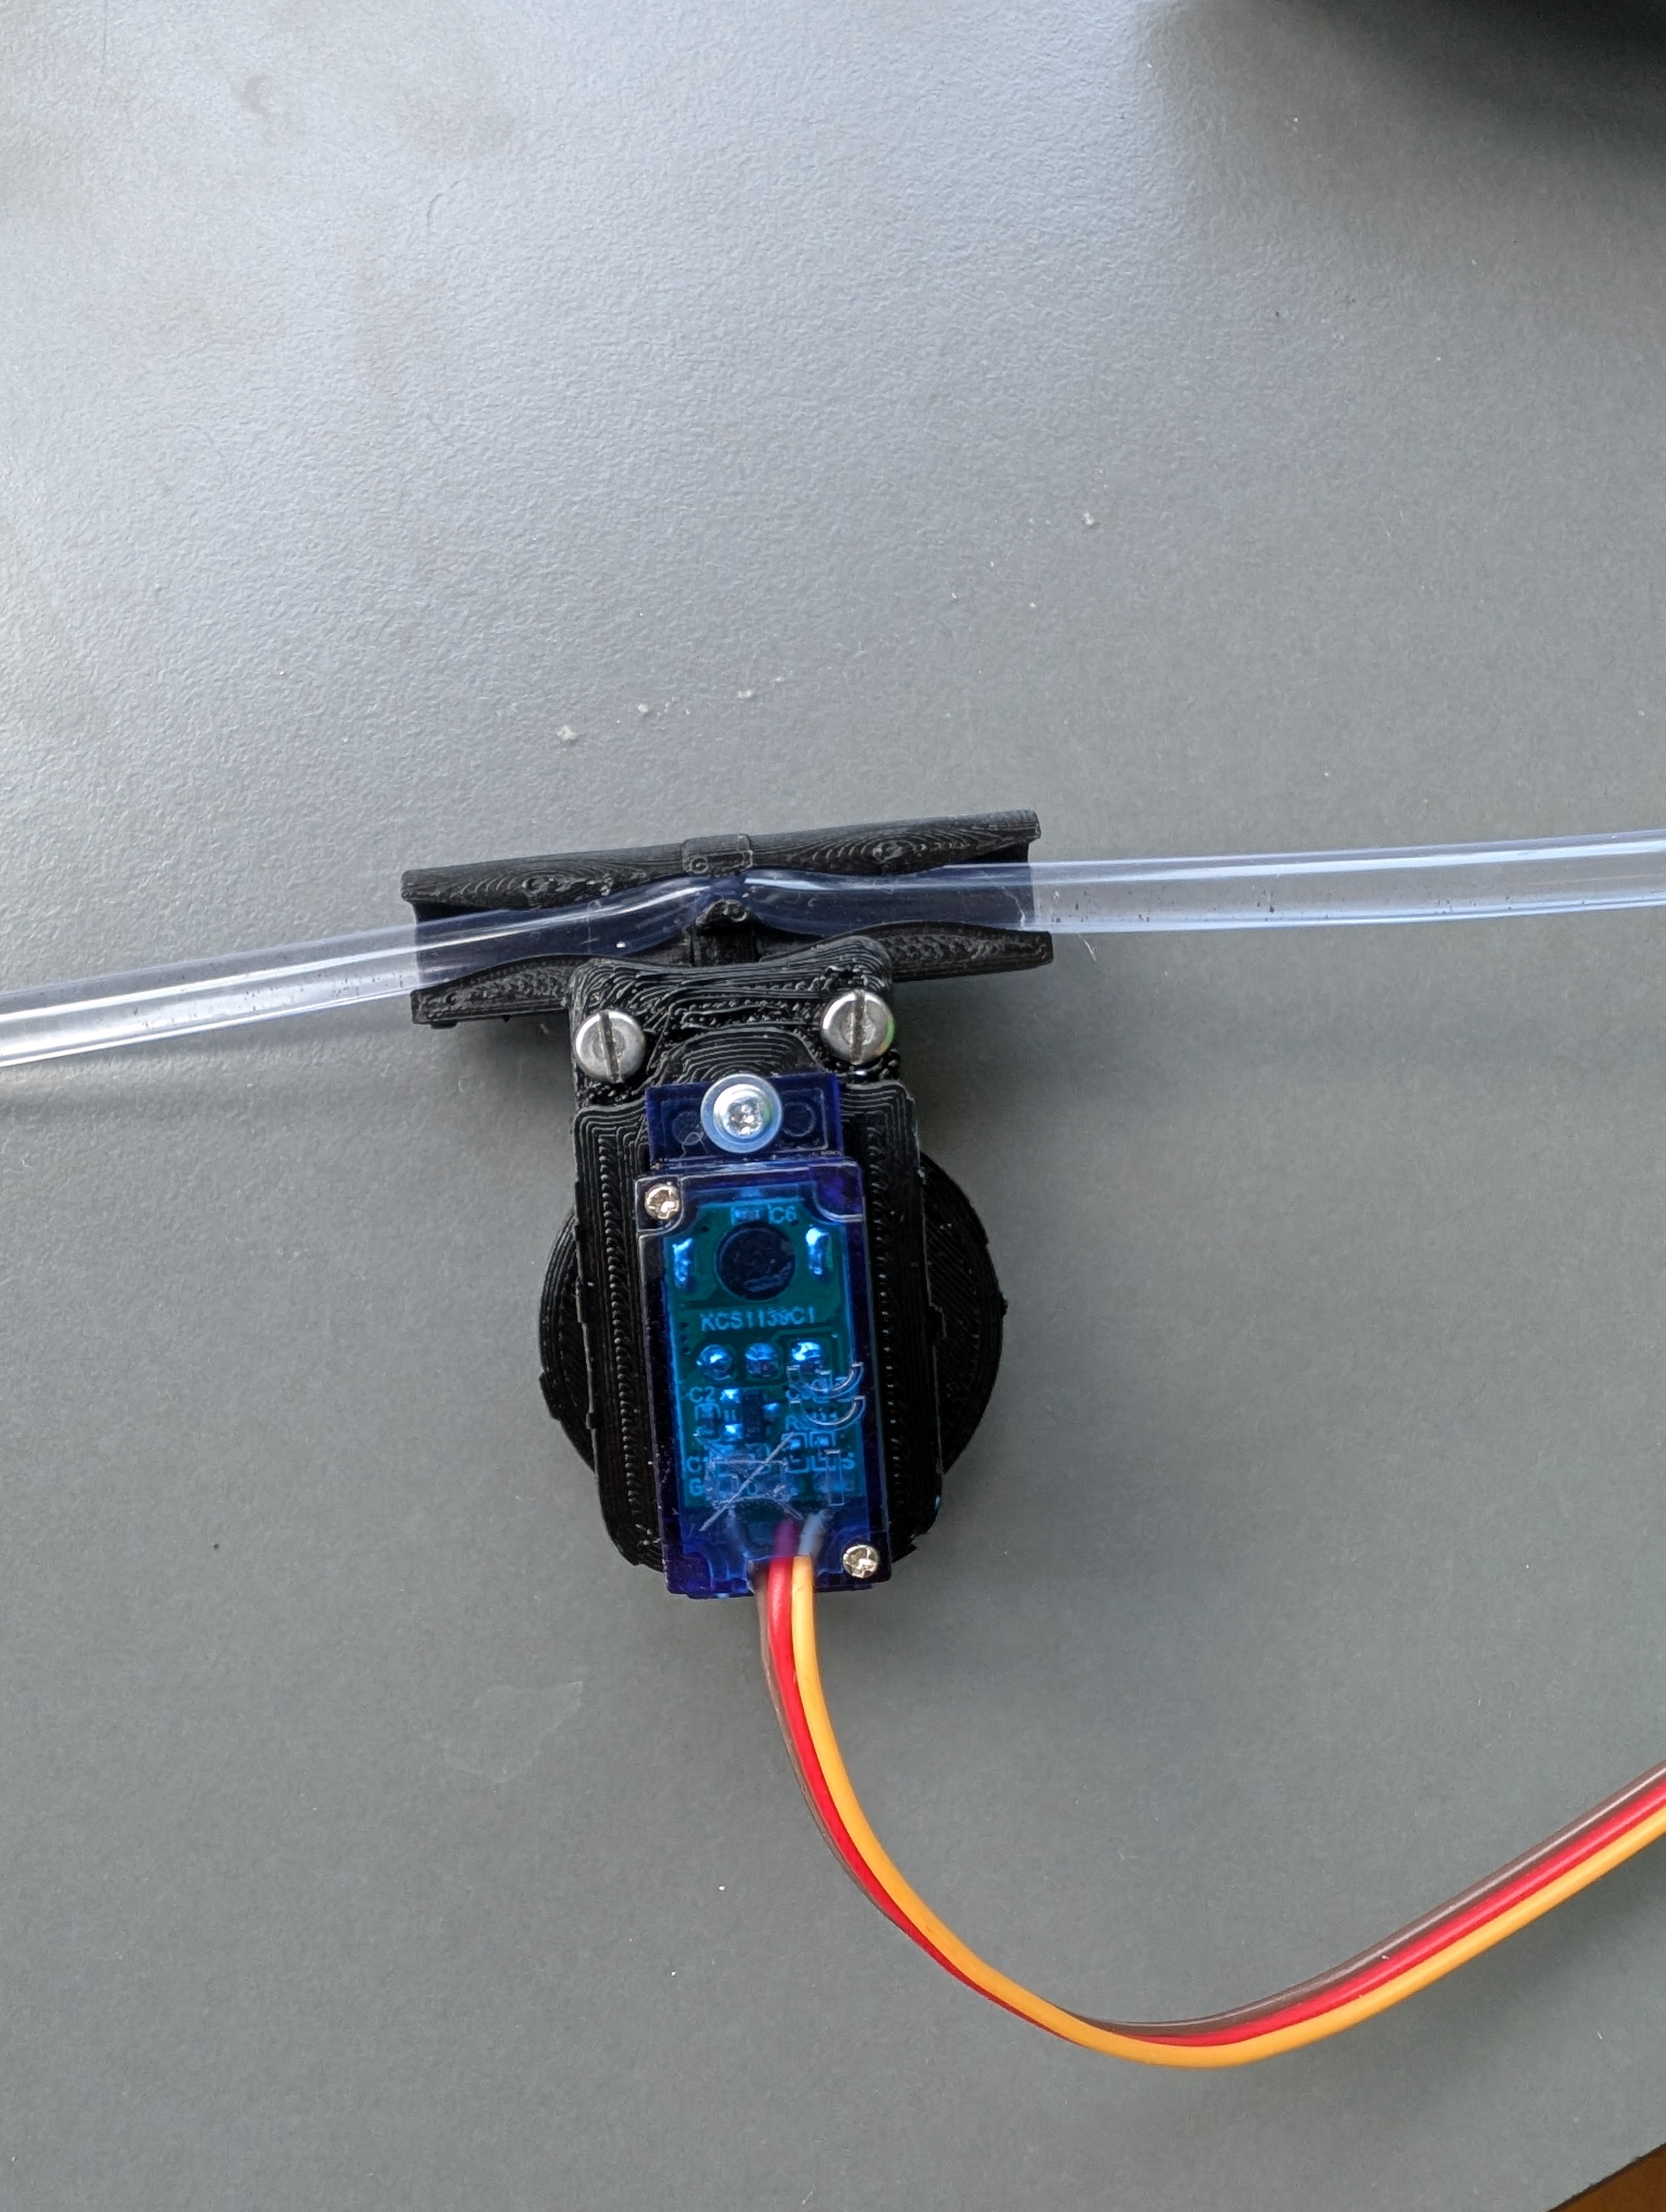
\includegraphics[width=0.3\textwidth]{Servo.jpg}
    \caption{Image of servo in the watering mechanism}
    \label{fig:servo}
\end{figure}

\section{Preliminary GUI}

\begin{figure}[H]
    \centering
    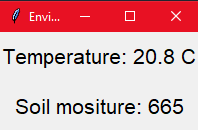
\includegraphics[width=0.3\textwidth]{Dummy Readings.png}
    \caption{GUI displaying simulated sensor readings}
    \label{fig:prelim_GUI_readings}
\end{figure}

\begin{figure}[H]
    \centering
    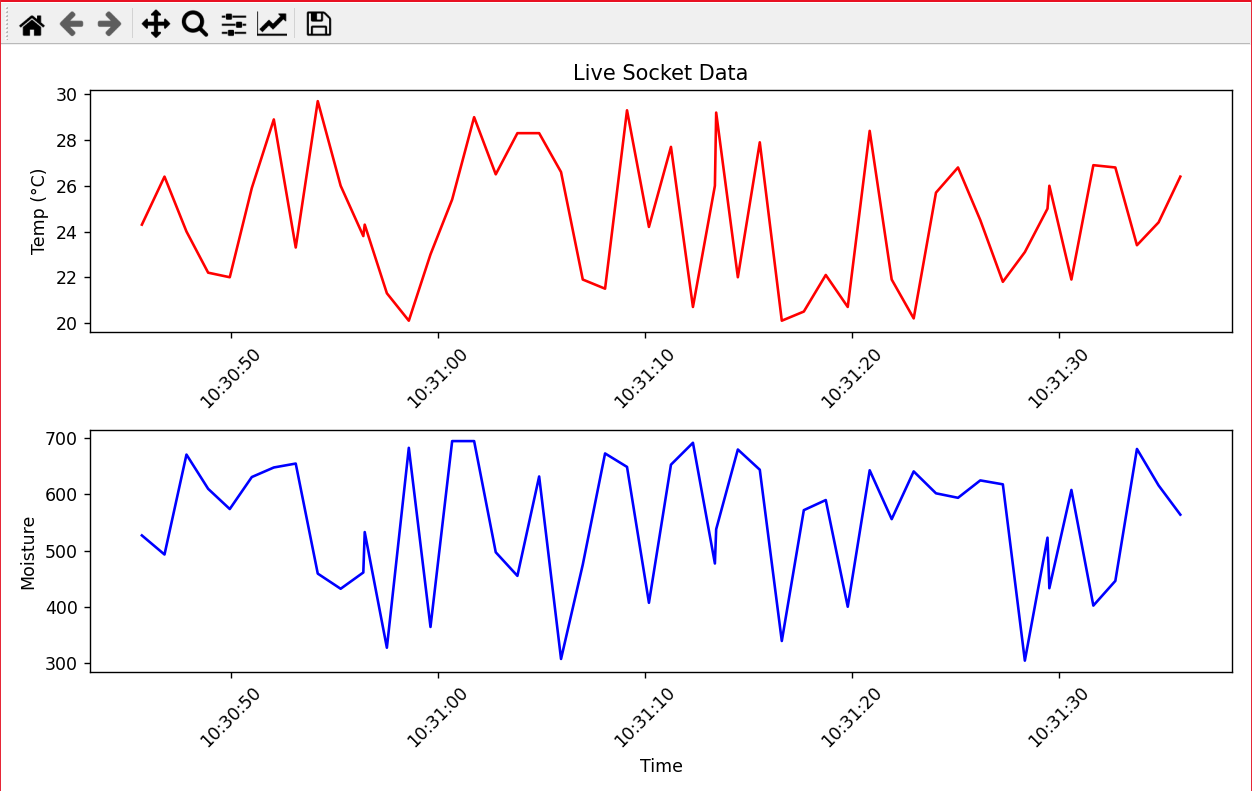
\includegraphics[width=0.8\textwidth]{Dummy Plotting.png}
    \caption{GUI displaying simulated plot of sensor readings}
    \label{fig:prelim_GUI_plot}
\end{figure}

\section{Code}

\begin{lstlisting}[style=cpp-style, 
caption={\textit{parseWarningCommand} function, 
emblematic of similar functions in \texttt{main.ino}}, label={prog:warn}]
void parseWarningCommand(const String &command){
    if (!command.startsWith("SET_WARN "))
        return;

    String rest = command.substring(9); // Remove "SET_WARN "
    int firstSpace = rest.indexOf(' ');
    int secondSpace = rest.indexOf(' ', firstSpace + 1);

    if (firstSpace == -1 || secondSpace == -1)
        return;

    String sensor = rest.substring(0, firstSpace);
    float minVal = rest.substring(firstSpace + 1, secondSpace).toFloat();
    float maxVal = rest.substring(secondSpace + 1).toFloat();

    if (sensor == "temp_C")
    {
        temp_warn_min = minVal;
        temp_warn_max = maxVal;
        Serial.println("Temp warning limits updated");
    }
    else if (sensor == "moisture")
    {
        minVal = constrain(minVal, 0, 100);
        maxVal = constrain(maxVal, 0, 100);
        moist_warn_min = (int)minVal;
        moist_warn_max = (int)maxVal;
        Serial.println("Moisture warning limits updated");
    }}
\end{lstlisting}

\begin{lstlisting}[style=cpp-style, 
caption={LED warning light}, label={prog:LED}]
void updateWarningLED(){
    // If warning active, activate pin 3 for LED
    if ((temp_warn_min != -999 && temp_warn_max != 999 &&
        (tmp_conv(analogRead(PIN_TMP36)) < temp_warn_min || tmp_conv(analogRead(PIN_TMP36)) > temp_warn_max)) ||
        (moist_warn_min != -1 && moist_warn_max != 1024 &&
        (convertMoistureToPercent(analogRead(PIN_MOIST) * (ADC_VREF / 5)) < moist_warn_min ||
        convertMoistureToPercent(analogRead(PIN_MOIST) * (ADC_VREF / 5)) > moist_warn_max)))
    {
        digitalWrite(LED_WARN, HIGH);
    }
    else
    {
        digitalWrite(LED_WARN, LOW);
    }}
\end{lstlisting}

\section{GUI}

\begin{figure}[H]
    \centering
    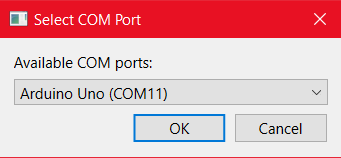
\includegraphics[width=0.6\textwidth]{1 - Select Comm Port.png}
    \caption{GUI displaying automatic Com port selection}
    \label{fig:port}
\end{figure}

\begin{figure}[H]
    \centering
    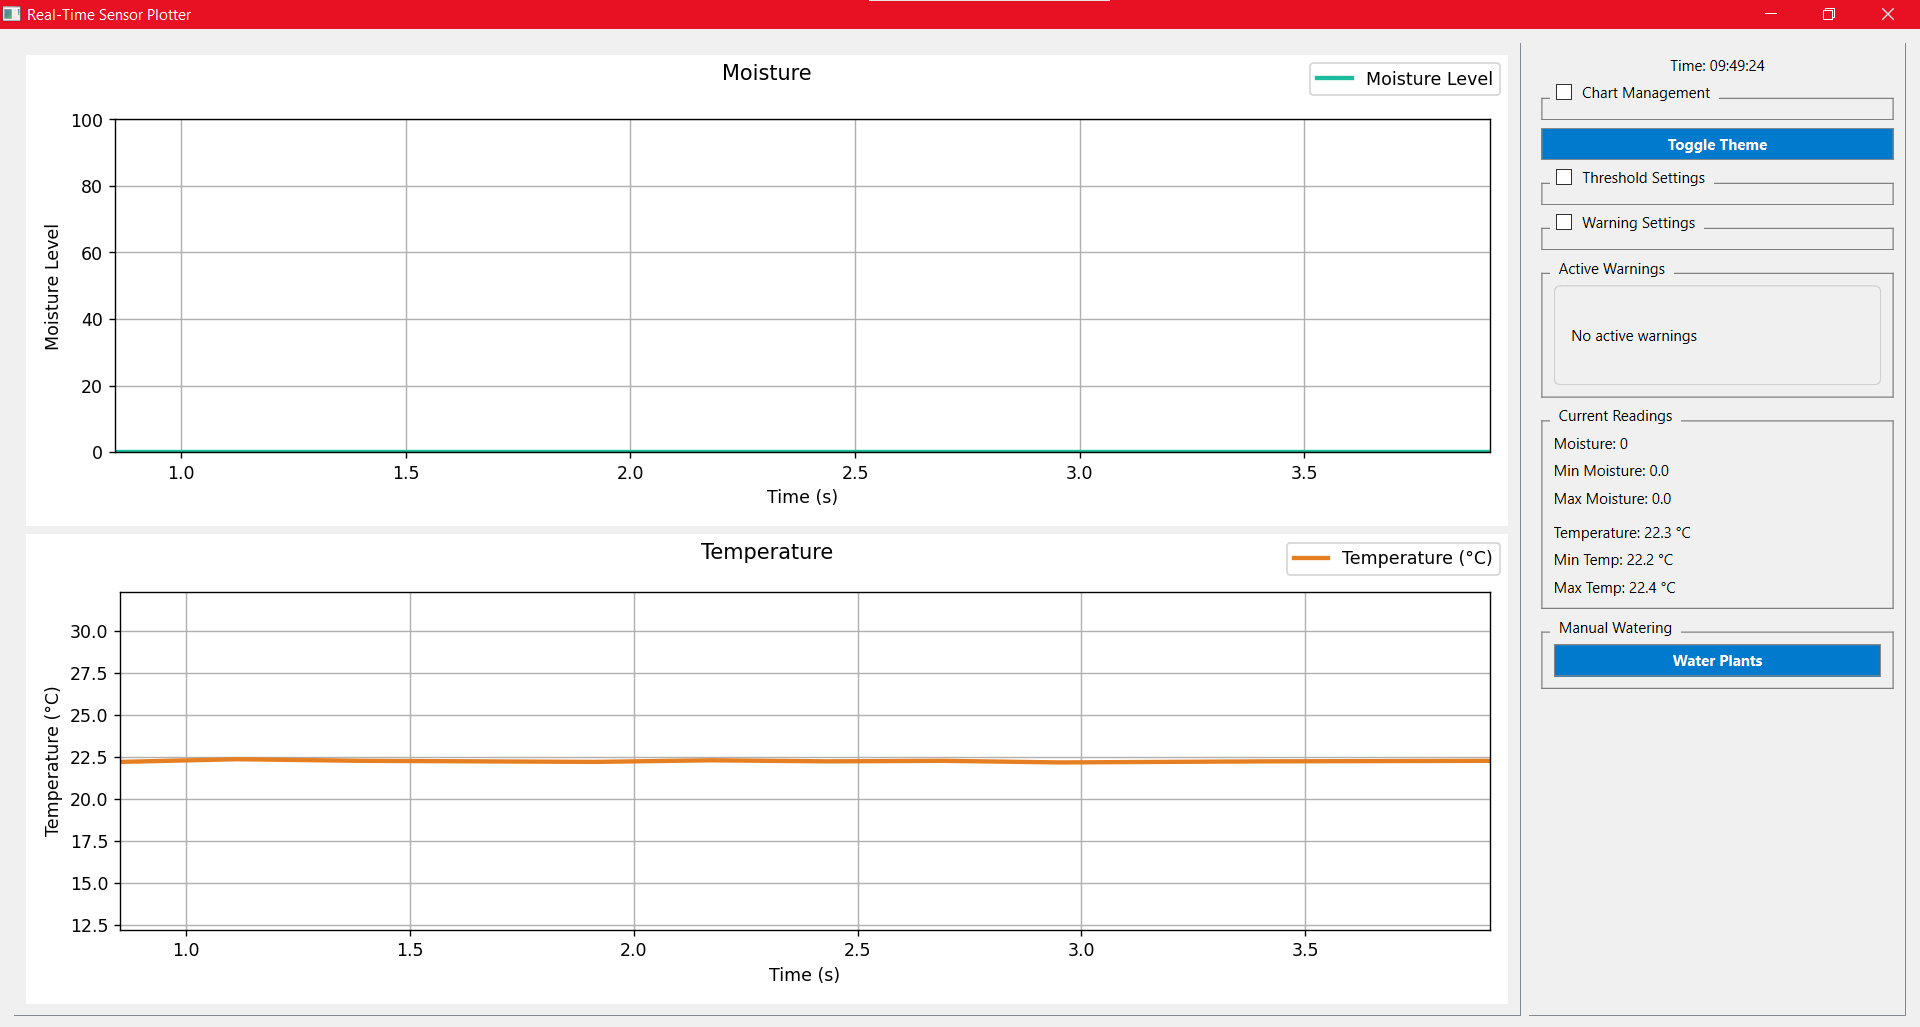
\includegraphics[width=0.8\textwidth]{2 - Blank Chart.png}
    \caption{The basic GUI}
    \label{fig:blank_gui}
\end{figure}

\begin{figure}[H]
    \centering
    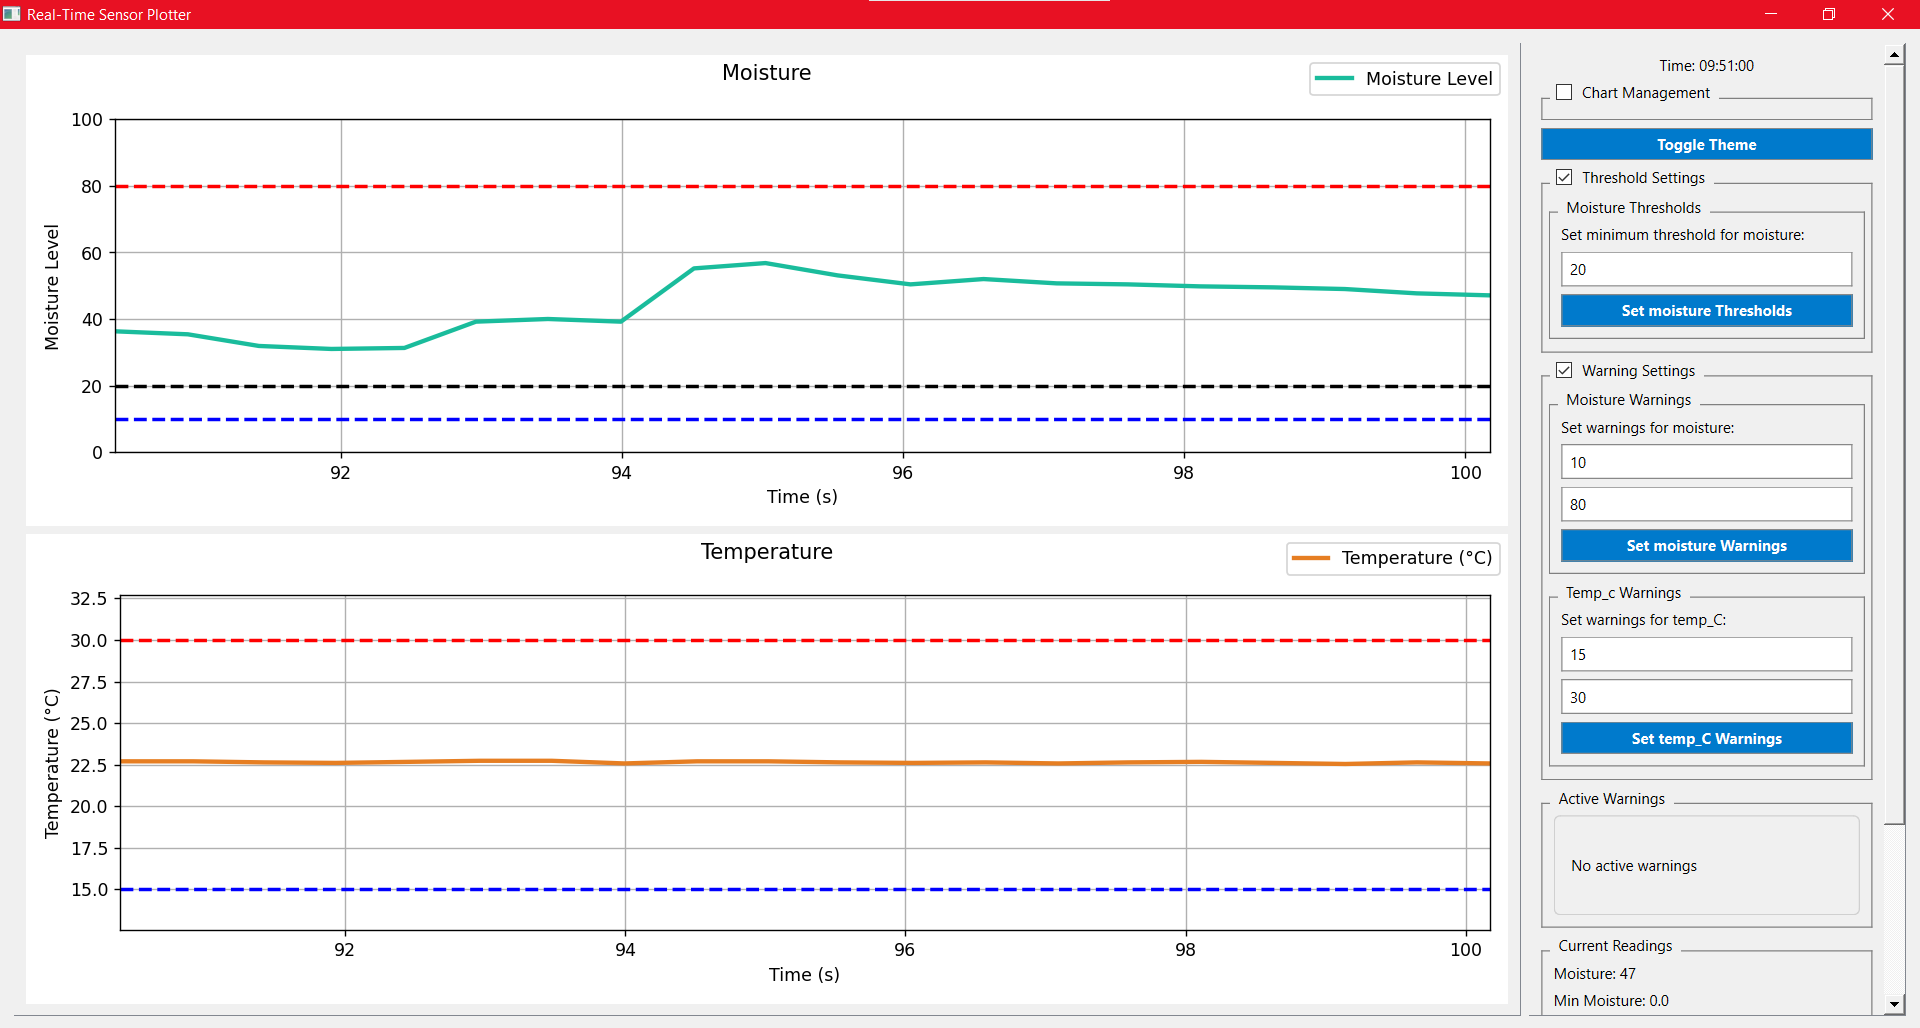
\includegraphics[width=0.8\textwidth]{3 - Threshold Setting.png}
    \caption{GUI displaying plotted data - including threshold and warnings}
    \label{fig:plotted}
\end{figure}

\begin{figure}[H]
    \centering
    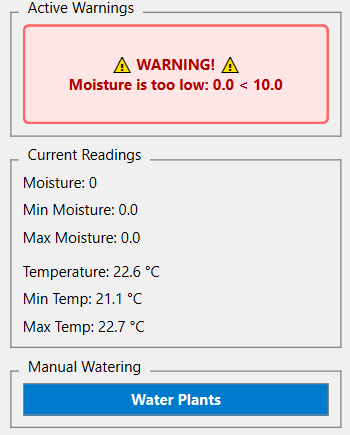
\includegraphics[width=0.4\textwidth]{4 - Warning.png}
    \caption{GUI displaying warning block}
    \label{fig:warning_block}
\end{figure}

\section{Interim Report}
\includepdf[pages=3-]{Reports/First Interim Report.pdf} % e.g. [pages={1,3-5,7}] to include pages 1,3,4,5,7
% Featuring the Interim Report

\end{document}